%%%%%%%%%%%%%%%%%%%%%%%%%%%%%%%%%%%%%%%%%%%%%%%%%%%%%%%%%%%%%%%%%%
%%  ~ Trabajo de Fin de Grado - Universidad de Vigo (ESEI) ~    %%
%% Autor: Diego Enrique Fontán Lorenzo                          %%
%% Tutor: Miguel Ramón Díaz-Cacho Medina                        %%
%% Convocatoria: Julio 2020/21                                  %%
%% Título: Framework de automatización de auditorías Red Team   %%
%%%%%%%%%%%%%%%%%%%%%%%%%%%%%%%%%%%%%%%%%%%%%%%%%%%%%%%%%%%%%%%%%%

%%%%%%%%%%%%%%%%%%%%%%%%%%%%%
%% Introduction
%%%%%%%%%%%%%%%%%%%%%%%%%%%%%

\chapter{Introducción} \label{cap:introduccion}

En este capítulo se detalla el marco contextual sobre el que se presenta la realización del trabajo, así como la motivación asociada al mismo. Se describen después los objetivos perseguidos, la descripción técnica de la solución propuesta y los aspectos legales. Finalmente, se expone la estructura completa de la documentación.\n

%%%%%%%%%%%%%%%%%%%%%%%%%%%%%
%% Context
%%%%%%%%%%%%%%%%%%%%%%%%%%%%%

\section{Marco contextual} \label{sec:marcocontextual}

La seguridad informática se puede definir como el conjunto de técnicas que permiten a la organización asegurar la confidencialidad, integridad y disponibilidad de su sistema de información.\sn

La pandemia y el confinamiento han obligado a las empresas a digitalizarse. El uso de tecnologías de acceso remoto como RDP (\textit{Remote Desktop Protocol}) y VPN (\textit{Virtual Private Network}) ha crecido en un 41\% y 33\% \fig{servicios expuestos}, respectivamente, desde el inicio del brote del coronavirus (COVID-19) \cite{shodantrends}.\n

\begin{figure}[h]
     \centering
     \begin{subfigure}[b]{0.3\textwidth}
         \centering
         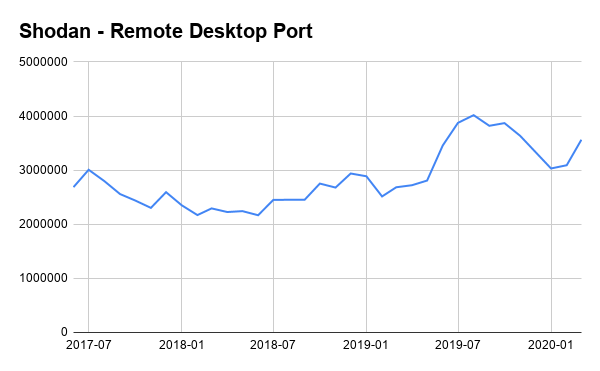
\includegraphics[width=\textwidth]{img/tables/01_Shodan-RDP.png}
         \caption{RDP expuesto.}
         \label{fig:puerto 3389 expuesto}
     \end{subfigure}
     \begin{subfigure}[b]{0.3\textwidth}
         \centering
         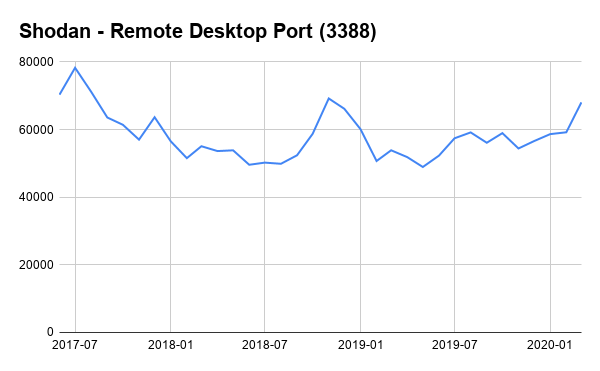
\includegraphics[width=\textwidth]{img/tables/02_Shodan-RDP-alt.png}
         \caption{RDP expuesto. (alt.)}
         \label{fig:puerto 3388 expuesto}
     \end{subfigure}
     \begin{subfigure}[b]{0.3\textwidth}
        \centering
        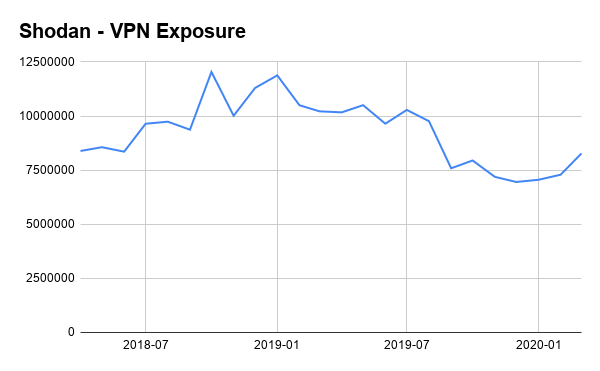
\includegraphics[width=\textwidth]{img/tables/03_Shodan-VPN.png}
        \caption{VPN expuesto.}
        \label{fig:servicio vpn expuesto}
     \end{subfigure}
    \caption{Cantidad de dispositivos según el servicio expuesto. Fuente: \textit{Shodan}.}
    \label{fig:servicios expuestos}
\end{figure}

La actual pandemia también ha tenido un gran impacto en la ciberseguridad. Los ataques informáticos contra corporaciones, así como las estafas en línea, se dispararon en más de un 400\% en marzo de 2020 en comparación con los meses anteriores, según la firma de abogados internacional \textit{Reed Smith} \cite{reedsmithcovidfraud}, mientras que \textit{Google} reveló que estaba bloqueando más de 18 millones de correos electrónicos de malware y phishing relacionados con el COVID-19 cada día \cite{googlecovidfraud}.\sn

Los ciberdelincuentes  siguen consiguiendo comprometer los datos y sistemas corporativos con relativa facilidad y de forma regular. Esto se debe a la falta de perfiles cualificados que sean capaces de realizar auditorías de seguridad (o \textit{pentestings}), con el fin de asegurar los activos de la compañía \cite{cybersecurityspecialist}. Además, las tácticas empleadas por los ciberdelincuentes son cada vez más sofisticadas, haciendo que este tipo de ejercicios se vuelvan a su vez más complejos y extensos. \textit{Gartner} ha proyectado que las empresas invirtieron más de 123.000 millones de dólares en ciberseguridad en 2020 \fig{cybersecuritybudget} y prevé que esa cifra aumente a 170.400 millones de dólares en 2022 \cite{cibersecuritybudget}.\n

\begin{figure}[h]
    \centering
    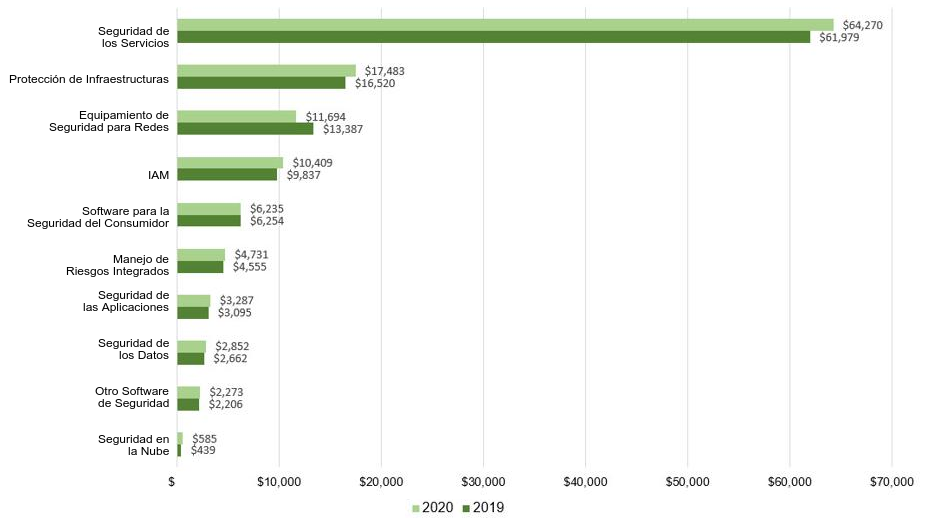
\includegraphics[width=15cm]{img/tables/04_Cybersecurity-Budget.png}
    \caption{Gasto mundial en ciberseguridad (en millones de dólares). Fuente: \textit{Forbes}.}
    \label{fig:cybersecuritybudget}
\end{figure}

%%%%%%%%%%%%%%%%%%%%%%%%%%%%%
%% Motivation
%%%%%%%%%%%%%%%%%%%%%%%%%%%%%

\section{Motivación} \label{sec:motivación}

La seguridad informática es un campo cambiante y en constante crecimiento. La complejidad a la hora de realizar ejercicios de intrusión requiere que los auditores tengan acceso a un amplio repertorio de herramientas, donde cada una de las cuales generalmente está enfocada en tareas concretas dentro de la totalidad de la auditoría.\sn

Además, el autor de este documento también ha experimentado la dificultad a la que se enfrenta un docente al intentar formar nuevos perfiles dentro del campo de la ciberseguridad.\sn

Esto se debe a que las soluciones \textit{software} actuales requieren de conocimientos informáticos avanzados, tienen una funcionalidad muy específica o sólo están disponibles para arquitecturas de sistemas concretos.



%%%%%%%%%%%%%%%%%%%%%%%%%%%%%
%% Objetives
%%%%%%%%%%%%%%%%%%%%%%%%%%%%%

\section{Objetivo} \label{sec:objetivos}

Este Trabajo de Fin de Grado se plantea con el objetivo de crear un proyecto de código abierto enfocado a la seguridad informática, que automatice y enlace varias de las etapas más habituales durante un \textit{pentesting} (listado de subdominios y servicios, comprobación de filtrados de información, credenciales por defecto, vulnerabilidades conocidas...), y que su uso sea válido tanto en auditorías reales como en entornos educativos, con el fin de simplificar y desmitificar las actividades relacionadas con el mundo de la ciberseguridad, acorde a lo detallado en el apartado \ref{sec:motivación}.\n

\subsection{Objetivos específicos} \label{sub:objetivosespecificos}

Además de llevar a cabo el proyecto, existen una serie de especificaciones que ha de cumplir el programa. Dichos requisitos, detallados a continuación, son necesarios para asegurarse de que la funcionalidad es acorde a la motivación inicial por parte del autor.\sn

\subsubsection{Manejo visual e intuitivo} \label{subsub:objvisual}

Debido a que una de las motivaciones de este proyecto es acercar el mundo de la ciberseguridad a aquellos perfiles ajenos al sector, es necesaria la opción de poder prescindir de la habitual línea de comandos. Una alternativa es reemplazarla por una interfaz gráfica, teniendo como preferencia un diseño similar a un lenguaje de programación visual. Como ejemplo de lenguajes visuales, se encuentran aquellas basadan en bloques (véase \textit{Scratch}\footnote{\url{https://scratch.mit.edu/}} o \textit{AppInventor}\footnote{\url{https://appinventor.mit.edu/}}), o basadas en nodos (\textit{Node-RED}\footnote{\url{https://nodered.org/}} o \textit{vvvv}\footnote{\url{https://vvvv.org/}}), entre otros, siendo este último la preferencia.\sn

Además, se pretende que al aproximarse a este concepto, la aplicación ofrezca una experiencia de usuario similar a la de ``crear recetas'', pudiendo compartirlas y reduciendo así el tiempo requerido para realizar auditorías de seguridad.\sn

\subsubsection{Estandarización de tareas} \label{subsub:objapi}

Se requiere que la aplicación ejecute tareas repetitivas, pertenecientes a las diferentes etapas de una auditoría de ciberseguridad, que interactúan directamente con servicios y dispositivos externos.\sn

Para ello, será necesaria la creación de una \textbf{Interfaz de Programación de Aplicaciones} (\textit{API} en adelante). Proporcionará una manera sencilla de realizar dichas tareas mediante llamadas estandarizadas a la aplicación, independientemente del servicio o dispositivo auditado.\sn

\subsubsection{Distribución sencilla} \label{subsub:objdist}

Acorde a la motivación mencionada en el apartado \ref{subsub:objvisual}, se requiere que la distribución de la aplicación sea lo más sencilla posible. Para ello, se tendrá como objetivo la compilación de todo el entorno en un único ejecutable, sin dependencias, y con soporte para los sistemas operativos y arquitecturas más populares.\sn

Este aspecto también concuerda con la ideología de crear un programa que sirva de reemplazo para gran parte de las soluciones existentes actualmente en el mercado, al poder ejecutar varias de las tareas habituales durante una auditoría de seguridad desde una misma plataforma que no dependa de programas externos.\n

%%%%%%%%%%%%%%%%%%%%%%%%%%%%%
%% Technical description
%%%%%%%%%%%%%%%%%%%%%%%%%%%%%

\section{Descripción técnica} \label{sec:desctecnica}

En este punto se especifican, de manera breve, los componentes que formarán la aplicación con el fin de contextualizar los siguientes capítulos. Los requisitos serán explicados en profundidad en los apartados \ref{sec:userrequirements} y \ref{cap:requirements}, así como la arquitectura y el diseño de la misma (apartados \ref{cap:arch} y \ref{cap:design}, respectivamente). La solución propuesta en este documento constará, según la naturaleza de sus componentes, de varios elementos.\sn

Si aplicamos una categorización basada en soluciones software con interfaz gráfica, podemos diferenciar la aplicación en dos partes: la \textbf{interfaz} (o \textit{frontend}) y el \textbf{servidor} (o \textit{backend})\footnote{Puede ser objeto de debate definir a qué categoría pertenece cada uno de los elementos que conforman la aplicación. En este documento, se atribuyen al \textit{frontend} todos aquellos elementos desarrollados mediante el uso de \textit{HTML}, \textit{CSS} y/o \textit{JavaScript}. El resto, se asocian con el \textit{backend}.}.\sn
 
Por otro lado, siguiendo una categorización enfocada en la utilidad, podemos diferenciar tres entidades \fig{mockuputility}:\sn

\begin{figure}[H]
    \centering
    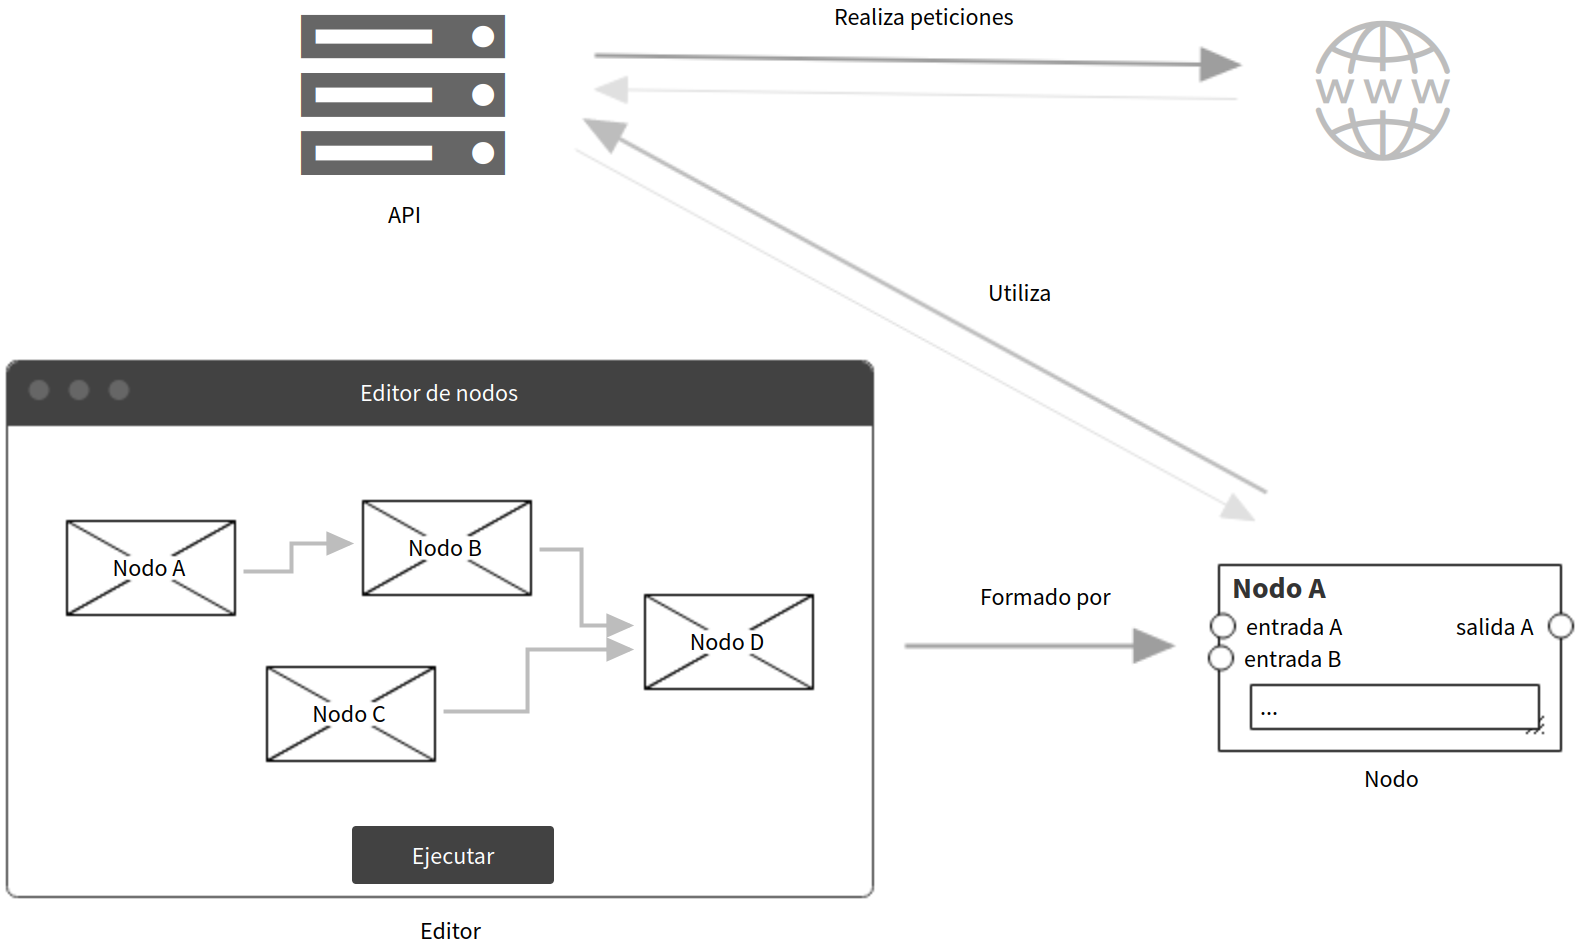
\includegraphics[width=11cm]{img/tables/05_Mockup-Utility.png}
    \caption{\textit{Mockup} según la utilidad de los componentes.}
    \label{fig:mockuputility}
\end{figure}


- La \textbf{\textit{API}}, encargada de manejar las peticiones y proporcionar los datos referentes a sistemas externos a la aplicación.\sn

- Los \textbf{nodos}, encargados de encapsular tareas concretas, de las cuales se pueden obtener datos a través de ciertos valores de entrada y/o parámetros de configuración (similar a la idea de \textit{función} dentro de la programación).\sn

- El \textbf{editor de nodos}, encargado de interpretar los nodos, interconectarlos entre si, manejar el flujo de datos y controlar la ejecución del programa.\n

Además, los componentes (así como la solución final) deberán cubrir una serie de características técnicas detalladas a continuación.

\subsection{Interfaz de Programación de Aplicaciones / API} \label{sub:api}

La \textbf{API} es, posiblemente, una de las partes más delicadas en cuanto a su diseño se refiere. Será la encargada de interactuar con los activos auditados, por lo que su implementación deberá ser precisa para evitar conexiones innecesarias y/o pérdidas en el contenido de los datos recibidos. Un mal diseño no sólo ralentizaría el servicio, sino que podría sobreexponer al auditor, además de causar daños sobre los activos.\sn

Muchas de las tareas habituales durante una auditoría de ciberseguridad no requieren de una conexión activa. Es por ello que las peticiones realizadas deberán cerrarse una vez finalizadas. En el caso de que se exija más información sobre el mismo activo se podrán reusar, siempre que sea posible, las respuestas entre las tareas que auditen características similares. De esta forma se consigue evitar la sobrecarga.\sn

La ejecución de las rutinas encargadas de realizar las conexiones se estandarizarán usando el protocolo \textit{HTTP}. Ésto se podrá conseguir mediante la creación de un servicio que tramite cada una de las peticiones y devuelva los resultados en formato \textit{JSON}.\sn

Para abarcar de manera satisfactoria estos problemas, se pretende utilizar un lenguaje de programación con acceso a librerías que permitan la creación de tramas a bajo nivel. De esta forma, se logrará obtener un mayor control sobre los datos enviados.\sn

Por otro lado, la velocidad de ejecución es un tema a tener en cuenta, dado que se realizarán múltiples tareas en un periodo de tiempo limitado. Por lo tanto, el lenguaje seleccionado debe ser compilado (dado que ofrece un mayor rendimiento frente a las alternativas interpretadas), y con soporte para modelos de computación no secuenciales (\textit{concurrencia} o \textit{paralelismo}, por ejemplo).\sn

También se pretende minimizar el riesgo de errores durante la ejecución, por lo que el lenguaje ha de ser \textit{tipado} (variables con tipos definidos) y que ofrezca mecanismos de gestión de excepciones.\sn

Ejemplos de lenguajes de programación que cumplen con estos requisitos son, entre otros: \textit{C/C++}, \textit{Rust} o \textit{Golang}.

\subsection{Editor de nodos} \label{sub:nodeeditor}

Este componente tendrá que encargarse de interpretar correctamente los nodos que lo conforman. Permite, a su vez, realizar operaciones de conexión y desconexión entre dos o más nodos, así como la personalización de los valores asociados a cada uno de ellos.\sn

El diseño seleccionado para el editor seguirá el paradigma de programación de flujo de datos (o \textit{dataflow programming}), el cual modela un programa como un gráfico dirigido en el que los datos fluyen entre las operaciones.\sn

Aunque existen varios patrones de diseño relacionados con este paradigma, se valorarán principalmente dos de ellos para la implementación: los basados en un único flujo de datos unidimensional (totalmente lineal), y los basados en nodos interconectados entre sí, formando un gráfico bidimensional con varios flujos de datos simultáneos \fig{mockupdataflow}.\sn

\begin{figure}[h]
    \centering
    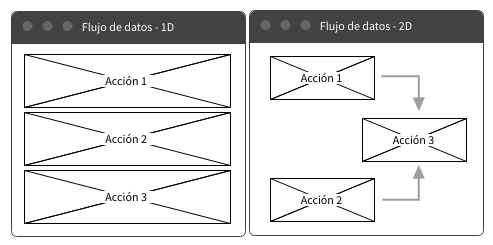
\includegraphics[width=10cm]{img/tables/06_Mockup-Dataflow-Types.png}
    \caption{\textit{Mockup} según el patrón de diseño.}
    \label{fig:mockupdataflow}
\end{figure}
\vspace{0.3cm}

Las aplicaciones con diseños unidimensionales\footnote{Un ejemplo de esta implementación es \textit{Cyberchef} (\url{https://gchq.github.io/CyberChef/})} son más intuitivas al compartir los datos en una única dirección, pero exige que todas las acciones sean evaluadas en el orden definido, existiendo un solo flujo de ejecución.\sn

Por el contrario, las soluciones con diseños bidimensionales ofrecen un mayor control sobre el orden de ejecución, pero su implementación requiere de un mayor esfuerzo, debido a que es necesario controlar excepciones tales como bucles infinitos, acciones huérfanas o flujos de datos independientes, entre otras \fig{mockupdataflowerrors}.\sn

\begin{figure}[H]
    \centering
    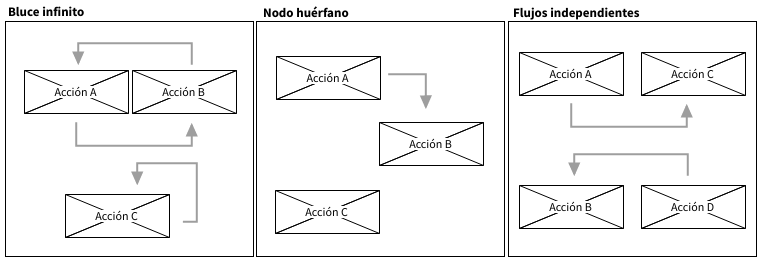
\includegraphics[width=11cm]{img/tables/07_Mockup-Dataflow-Problems.png}
    \caption{\textit{Mockup} de errores comunes al desarrollar diseños bidimensionales.}
    \label{fig:mockupdataflowerrors}
\end{figure}

Para la implementación de este diseño, es necesario que el lenguaje de programación seleccionado conste de librerías que permitan el desarrollo de interfaces altamente personalizables. Los lenguajes como \textit{Golang} o \textit{Rust}, mencionados en el apartado \ref{sub:api}, carecen de dichas librerías\footnote{Algunos de ellos ni siquiera ofrecen soporte gráfico, como \textit{Rust}. (\url{https://www.areweguiyet.com/})}, por lo que también se valorará realizar la interfaz mediante lenguajes web.\sn

Los nodos deberán seguir un estándar y ofrecer la capacidad de definir nuevos a través del uso de archivos parametrizados que consten, por ejemplo, de los siguientes valores:\sn

- \textbf{Identificador}: Cadena única usada para referenciar al nodo.

- \textbf{Nombre}: Texto identificativo mostrado en el editor.

- \textbf{Categoría}: Grupo al que pertenece según su funcionalidad.

- \textbf{Descripción}: Documentación relativa a su utilidad.

- \textbf{Etiquetas}: Palabras descriptivas por las que filtrar al nodo.

- \textbf{Entradas}: Valores de entrada requeridos.

- \textbf{Salidas}: Valores resultantes de la ejecución del nodo.

- \textbf{Controles}: Parámetros de configuración.

- \textbf{Código}: Método utilizado para generar los valores de salida.\sn

Los flujos de datos también deberán poder exportarse e importarse mediante ficheros, los cuales especificarán, al menos:\sn

- \textbf{Identificador}: Cadena usada para referenciar los tipos de nodos soportados.

- \textbf{Nodos}: Resumen de los nodos presentes en el editor, así como las conexiones entre ellos.\n

\subsection{Binario precompilado multiplataforma} \label{sub:binary}

De acuerdo al objetivo detallado en el punto \ref{subsub:objdist}, la aplicación ha de ser fácil de distribuir. Para ello, será necesario que el lenguaje seleccionado sea capaz de procesar plantillas \textit{HTML}. Dichas plantillas formarán parte del código fuente, con la intención de reducir el número de archivos que formen la aplicación a un único fichero ejecutable. Además, esto requiere que sea un lenguaje compilado, al igual que en el apartado \ref{sub:api}.\sn

Por otro lado, el programa ha de ser multiplataforma y sin dependencias de librerías o programas externos.\sn

Existen compiladores (como el nativo de \textit{Golang}) que permiten generar binarios teniendo como objetivo cualquier sistema operativo y plataforma, independientemente de la arquitectura del sistema anfitrión.\n

%%%%%%%%%%%%%%%%%%%%%%%%%%%%%
%% Laws
%%%%%%%%%%%%%%%%%%%%%%%%%%%%%

\section{Aspectos legales} \label{sec:legal}

A continuación se detallan los aspectos legales asociados al proyecto. Debido a la naturaleza del mismo, \textbf{el uso de la aplicación resultante puede ser un acto constitutivo de delito}, según la regulación de cada país.\sn

En España, se entiende por \textbf{Delito Informático} todo aquel ataque que se produce contra el derecho a la intimidad, delitos de descubrimiento y revelación de secretos mediante el apoderamiento y difusión de datos reservados registrados en ficheros o soportes informáticos. (\textit{Art.197-201 Código Penal} \cite{LO1995}).\sn

Concretamente, considera delito de \textbf{sabotaje informático} a toda aquella acción que produzca daños mediante la destrucción o alteración de datos, programas o documentos electrónicos contenidos en redes o sistemas informáticos (\textit{Art. 263} \cite{LO1995}), y delito de \textbf{fraude informático} a las estafas a través de la manipulación de datos o programas para la obtención de un lucro ilícito (\textit{Art. 248}\cite{LO1995}).\sn

Además, en la reforma realizada en 2010 \cite{LO2010}, la detección de vulnerabilidades informáticas se considera acto de delito. Cualquier persona que detecte vulnerabilidades en aplicaciones o sitios web, sin consentimiento explícito de los interesados, puede acabar con consecuencias legales. En otras palabras, \textbf{realizar un acceso no consentido, sin autorización, será considerado hecho válido de sanción, aunque no exista intención de cometer un delito}. El usuarios que comete el acto puede ser sancionado con una pena de prisión de entre seis meses y dos años.\sn

Las personas jurídicas dedicadas a la seguridad informática deben conocer esta ley, y todas las consecuencias que pueden ocurrir en el incumplimiento de la misma. Es recomendable que cualquier individuo al cargo de una auditoría de seguridad sea informado y tenga consciencia de ello, entendiendo el ámbito en el que se encuentra y a las leyes que está sujeto. Actualmente, el Código Penal no hace distinción entre un investigador de seguridad que actúa sin consentimiento y un delincuente que se aprovecha de las vulnerabilidades para obtener beneficio propio.\sn

Respecto al uso de la aplicación producto del proyecto, \textbf{el autor de este documento no se hace responsable en caso de que se presenten cargos penales contra cualquier individuo o corporación que utilice la herramienta en contra de las leyes estipuladas}, así como de los daños causado por un mal uso de la misma. Es responsabilidad del usuario final obedecer todas las leyes aplicables.\sn

Se recomienda que su uso sea limitado a entornos controlados, tales como entornos educativos, y/o pruebas de intrusión bajo autorización previa de los interesados.\n

%%%%%%%%%%%%%%%%%%%%%%%%%%%%%
%% Structure
%%%%%%%%%%%%%%%%%%%%%%%%%%%%%

\section{Organización de la documentación} \label{sec:structure}

A continuación se detalla la documentación relativa al proyecto, así como su estructura.\sn

\subsection{Memoria del proyecto} \label{sub:memo}

Se trata del documento actual. En él se recogen formalmente todos los aspectos del proyecto, desde sus primeras fases, así como las decisiones arquitectónicas tomadas, el proceso completo de desarrollo, la documentación generada y las conclusiones a
las que se han llegado como consecuencia de la realización del ejercicio.\sn

Además, se adjuntan tres anexos correspondientes a:\sn

- \textbf{Anexo A}: La bibliografía consultada durante la investigación inicial.\sn

- \textbf{Anexo B}: El manual de usuario para la correcta instalación y uso del producto desarrollado.\sn

- \textbf{Anexo C}: Resumen de los controles típicos durante una auditoría de seguridad web según la metodología descrita en la \textit{OWASP Web Security Testing Guide}\cite{owaspwstg}.\n

\subsection{Documentación del código} \label{sub:codecomments}

El código de la aplicación se ha comentado detallando las funcionalidades de las partes más importantes.\sn

Es posible visualizar de forma \textit{online} a la documentación de las clases definidas en el apartado \ref{fig:classdiagramserver}. La \textit{URL} de acceso es: \url{https://pkg.go.dev/github.com/cosasdepuma/masterchef}.\sn

Por otro lado, se pone a disposición del usuario el archivo \textit{swagger.yml}. Esto permite documentar las llamadas a la \textit{API}, usando la tecnología descrita en el apartado \ref{sec:swagger}.\n

\subsection{Repositorio público} \label{sub:repo}

Debido a que éste es un proyecto de código abierto, todos los archivos a los que se hacen referencia en esta memoria se encuentran alojados en un repositorio público. Se puede consultar y realizar un seguimiento, a través de: \url{https://github.com/CosasDePuma/Masterchef}.